\documentclass[12pt]{article}

% Layout.
\usepackage[top=1in, bottom=0.75in, left=1in, right=1in, headheight=1in, headsep=6pt]{geometry}

% Fonts.
\usepackage{mathptmx}
\usepackage[scaled=0.86]{helvet}
\renewcommand{\emph}[1]{\textsf{\textbf{#1}}}

% TiKZ.
\usepackage{tikz, pgfplots}
\usetikzlibrary{calc}

% Misc packages.
\usepackage{amsmath,amssymb,latexsym}
\usepackage{graphicx}
\usepackage{array}
\usepackage{xcolor}
\usepackage{multicol}
\usepackage{fancyhdr}
\pagestyle{fancy}
\usepackage{adjustbox}
\usepackage{enumitem}

\usetikzlibrary{calc,trees,positioning,arrows,fit,shapes,through, backgrounds}
\usetikzlibrary{patterns}

\usetikzlibrary{decorations.markings}
\usetikzlibrary{arrows}

% Misc.
\renewcommand{\d}{\displaystyle}
\newcommand{\ds}{\displaystyle}
\def\bc{\begin{center}}
\def\ec{\end{center}}
\def\be{\begin{enumerate}}
\def\ee{\end{enumerate}}

\newcommand{\ans}[1][1in]{\rule{#1}{.5pt}}


\lhead{Math F113X: Quiz 4}

\begin{document}

\ 

%\vspace{.25cm}

\noindent \textbf{Name:} \hrulefill \quad  score:\ans[1cm] \ / 10 \\


There are 10 points possible on this quiz. No aids (book, notes, etc.)
are permitted. You may use a non-programmable calculator.  {\bf Show
all work and supporting calculations for full credit. Explain how you
get your answers.}



\be

% \item (3 pts. total -- 1 pt. each) Use the graph below to answer the following
%   questions.

\makeatletter
\newcommand{\Letter}[1]{\@Alph{#1}}
\makeatother



\item (5 pts.) Recall Kruskal's algorithm roughly says the
  following:
	
  \fbox{Kruskal's Algorithm} Select the cheapest edge in the graph
  that does not create a circuit. Stop when a spanning tree is
  obtained.\\

  Use Kruskal's Algorithm to find a minimum weight spanning tree in the
  graph below. Break ties by choosing the alphabetically earliest edge
  first.

  \bigskip
  \bigskip


  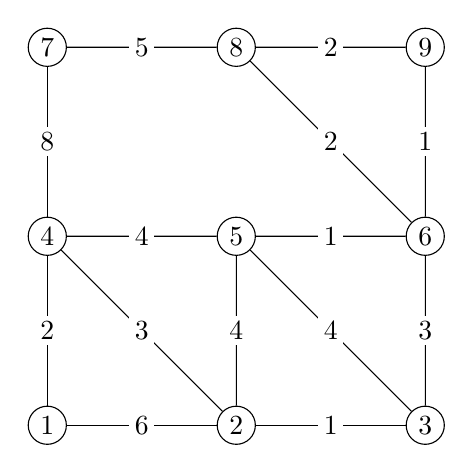
\begin{tikzpicture}[baseline=(current bounding
    box.center),lbl/.style={fill=white, inner sep = 2pt, }, scale = 1.2]
    \tikzstyle{vtx}=[circle, draw, inner sep=2pt]%, minimum size=6pt]
    \foreach \i in {0,1,2}{
      \path let \n1 = {int(\i+0)}, \n2 = {int(\i+0+1)} in node[vtx] (v\n1)
      at (2*\i,2*0){$\Letter{\n2}$};
      \path let \n1 = {int(\i+3)},\n2 = {int(\i+3+1)} in node[vtx] (v\n1) at
      (2*\i,2*1){$\Letter{\n2}$};
      \path let \n1 = {int(\i+6)},\n2 = {int(\i+6+1)} in node[vtx] (v\n1) at
      (2*\i,2*2){$\Letter{\n2}$};
    }
 
    \foreach \i/\j/\k in {0/1/6, 1/2/1, 0/3/2, 1/4/4, 2/4/4, 2/5/3, 3/4/4,
      4/5/1, 5/8/1, 5/7/2, 1/3/3, 3/6/8, 6/7/5, 7/8/2}{
      \draw (v\i) --node[lbl]{\k} (v\j);
    }

  \end{tikzpicture}
  %%
  \hfill
  \begin{tabular} {p{1.5cm}|c | c}
    used? & edges  & weights \\ \hline \hline
          &BC & 1\\ \hline
          &EF & 1\\ \hline
          &FI & 1\\ \hline
          &AD & 2\\ \hline
          &FH & 2\\ \hline
          &HI & 2\\ \hline
          &BD & 3\\ \hline
          &CF & 3\\ \hline
          &BE & 4\\ \hline
          &CE & 4\\ \hline
          &DE & 4\\ \hline
          &GH & 5\\ \hline
          &AB & 6\\ \hline
          &DG & 8
  \end{tabular}

  Draw the minimum weight spanning tree below.

  \vfill

  %%
  \begin{tikzpicture}[baseline=(current bounding
    box.center),lbl/.style={fill=white, inner sep = 2pt, }, scale = 1.2]
    \tikzstyle{vtx}=[circle, draw, inner sep=2pt]%, minimum size=6pt]
    \foreach \i in {0,1,2}{
      \path let \n1 = {int(\i+0)}, \n2 = {int(\i+0+1)} in node[vtx] (v\n1)
      at (2*\i,2*0){$\Letter{\n2}$};
      \path let \n1 = {int(\i+3)},\n2 = {int(\i+3+1)} in node[vtx] (v\n1) at
      (2*\i,2*1){$\Letter{\n2}$};
      \path let \n1 = {int(\i+6)},\n2 = {int(\i+6+1)} in node[vtx] (v\n1) at
      (2*\i,2*2){$\Letter{\n2}$};
    }
 

  \end{tikzpicture}

  \bigskip

  \bigskip


  What is the total weight of the spanning tree you found? \ans
	
  \vfill

  \newpage

  
\item Recall Dijkstra's algorithm roughly says the following:
  
\fbox{Dijkstra's Algorithm}

\begin{enumerate}[label=(\roman*)]
	\item  Mark the ending vertex with a distance of zero and label it as \emph{current}.\\
	(FYI: Once a \emph{current} vertex is explored, it will be labelled \emph{visited} and never considered again.)
	\item  Let $v$ be the current vertex. For every vertex $w$ with an edge to $v$ \emph{not marked as \textbf{visited}}, calculate the distance from $w$ to $e$ through $v.$ If this distance is smaller than the present distance, update $w$ with the new distance. Otherwise, do nothing. \\
	(FYI: This number is called the tentative distance to $e$.)
	\item Mark the current vertex as \emph{visited.} Never look at this vertex again.
	\item Identify the \emph{un-visited} vertex with the smallest distance to $e$. Mark it as current and return to step (ii). You know when to stop when vertex $s$ is labeled as \textbf{current}.
\end{enumerate}

  Use Dijkstra's Algorithm to determine the shortest (weighted)
  distance from vertex $A$ to vertex $G$.

\begin{adjustbox}{valign=t,minipage={.4\textwidth}}
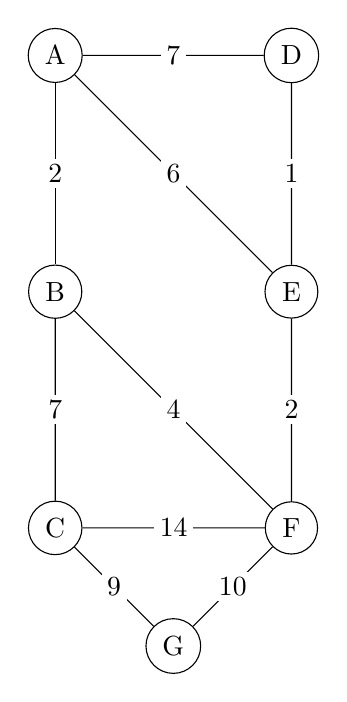
\begin{tikzpicture}[scale=1.5, lbl/.style={midway, fill=white, inner sep = 2pt}]
\node[draw, circle] (C) at (0,4) {B} ;
\node[draw, circle] (D) at (0,2) {C} ;
\node[draw, circle] (E) at (2,6) {D} ;
\node[draw, circle] (F) at (2,4) {E} ;
\node[draw, circle] (G) at (2,2) {F} ;
\node[draw, circle] (H) at (0,6) {A} ;
\node[draw, circle] (I) at (1,1) {G};

\draw (C) -- node[lbl]{7}(D) -- node[lbl]{9} (I);
\draw (E)  -- node[lbl] {1}(F)  -- node[lbl] {2} (G) -- node[lbl]{10} (I);
\draw (E) -- node[lbl] {7} (H) ;
\draw (F) -- node[lbl]{6} (H) ;\draw (H) -- node[lbl]{2} (C);
\draw (C) -- node[lbl]{4}(G) ;\draw (D) -- node[lbl]{14}(G);
% \draw (D) -- node[lbl] {8} (T);
% \draw (A) -- node[lbl]{3} (E);
% \draw (E) -- node[lbl]{6}(H);
\end{tikzpicture}
\end{adjustbox}
\begin{adjustbox}{valign=t,minipage={.25\textwidth}}
\begingroup
\renewcommand{\arraystretch}{1.5}
 \begin{tabular}{ |c | c |c| c|}
 \hline
 &&\textbf{tentative}&\\
 vertex & current/ & minimum& preceding\\ 
 &visited&\quad distance to $G$ \quad& vertex\\
 \hline
A&&& \\
\hline 
B&&& \\
\hline 
C&&& \\
\hline 
D&&& \\
\hline 
E&&& \\
\hline 
F&&& \\
\hline 
G&&& \\
\hline 
 \end{tabular}
\endgroup
\end{adjustbox}

\vfill


Length of the shortest path from $A$ to $G$: \underline{\hspace{1in}}\\

Find the shortest path from $A$ to $G$. The last column of the table
should support your answer.
\vfill

Path: \underline{\hspace{7cm}}
  
  

  \ee
\end{document}
%%% Local Variables:
%%% mode: LaTeX
%%% TeX-master: t
%%% End:
